\documentclass{article}
\usepackage[paperwidth=38cm,paperheight=26cm,margin=0.3cm]{geometry}
\usepackage{tikz}
\usepackage{amsmath}
\pagestyle{empty}
\begin{document}
\centering
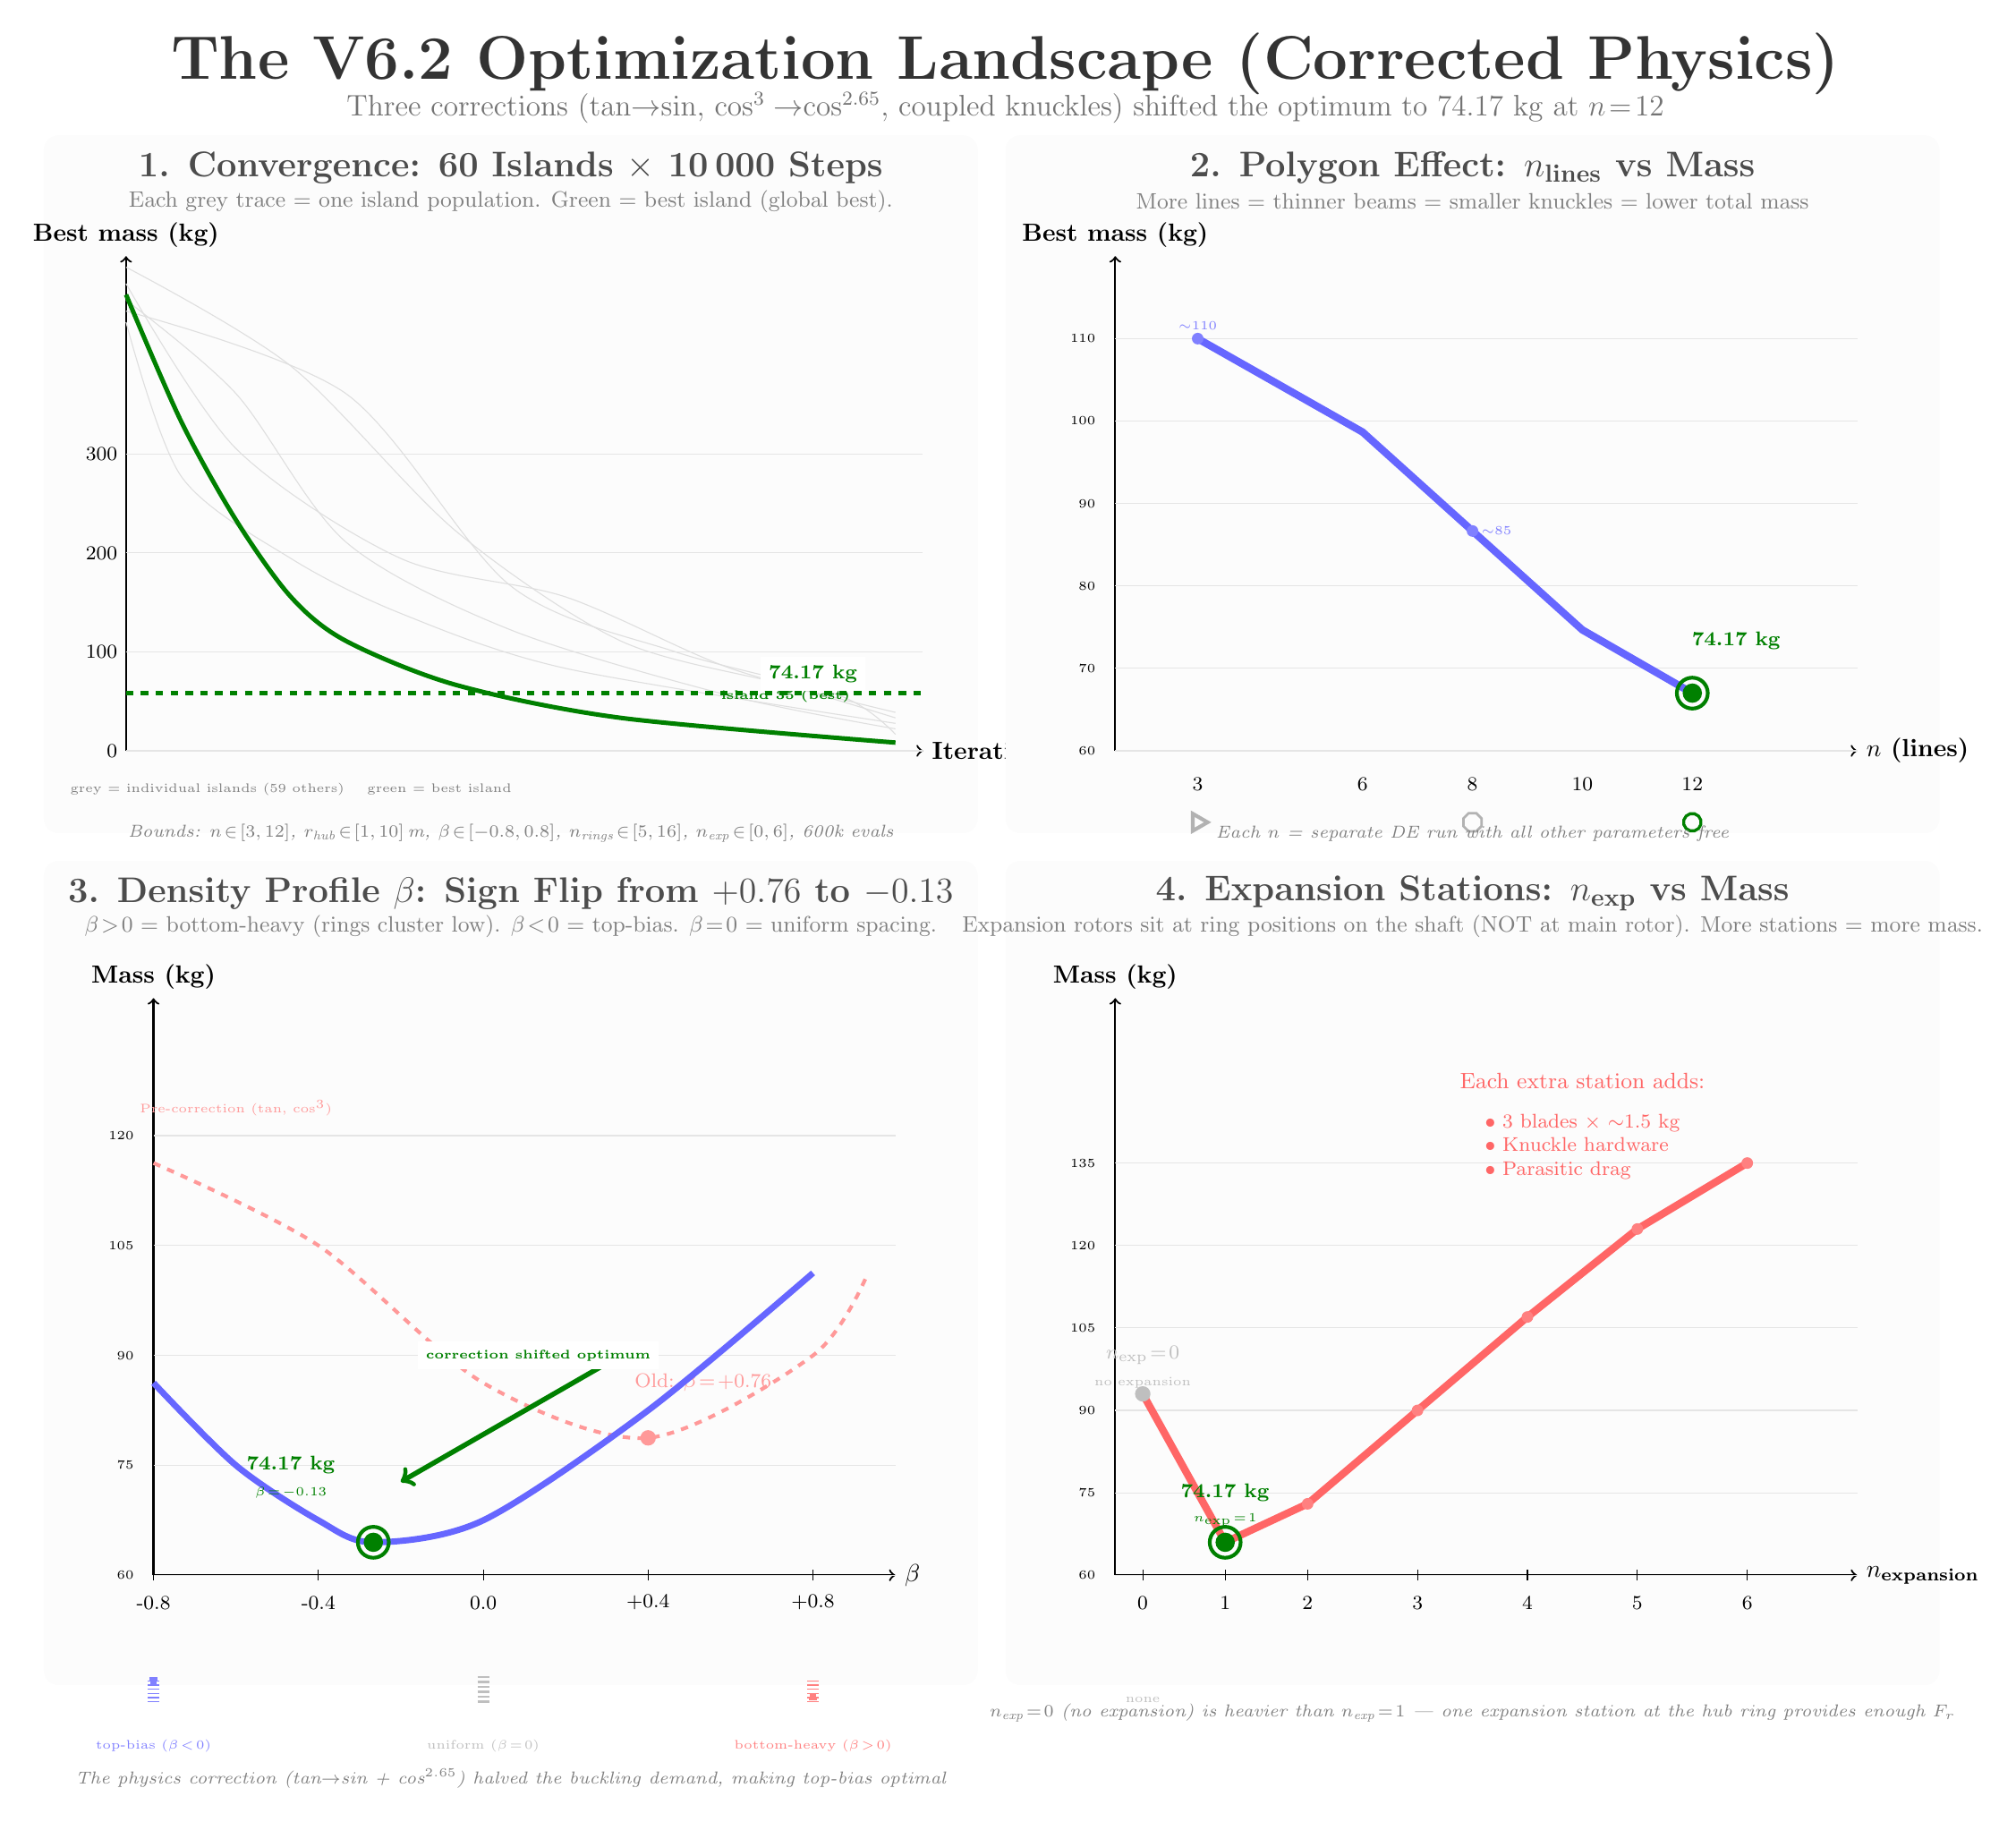
\begin{tikzpicture}[scale=0.78]

% === GLOBAL TITLE ===
\node[font=\bfseries\Huge, black!80] at (17.0,29.0) {The V6.2 Optimization Landscape (Corrected Physics)};
\node[font=\large, black!55] at (17.0,28.2) {Three corrections (tan$\rightarrow$sin, cos$^3\rightarrow$cos$^{2.65}$, coupled knuckles) shifted the optimum to 74.17 kg at $n\!=\!12$};

% ============================================================
% PANEL 1: Convergence History
% ============================================================
\begin{scope}[shift={(0,15.5)}]
  \fill[black!1, rounded corners=6pt] (-0.5,-0.5) rectangle (16.5,12.2);
  \node[font=\bfseries\Large, black!70] at (8.0,11.6) {1. Convergence: 60 Islands $\times$ 10\,000 Steps};
  \node[font=\small, black!50] at (8.0,11.0) {Each grey trace = one island population. Green = best island (global best).};

  \draw[->, thick] (1.0,1.0) -- (1.0,10.0) node[above, font=\bfseries] {Best mass (kg)};
  \draw[->, thick] (1.0,1.0) -- (15.5,1.0) node[right, font=\bfseries] {Iteration};

  \foreach \y/\label in {1.0/0,2.8/100,4.6/200,6.4/300} {
    \draw[gray!20] (1.0,\y) -- (15.5,\y);
    \node[left, font=\footnotesize] at (1.0,\y) {\label};
  }

  % Grey traces = individual islands
  \draw[gray!25, line width=0.4pt, smooth] plot coordinates {(1.0,9.2) (3.0,7.5) (5.0,4.8) (8.0,3.2) (12.0,2.0) (15.0,1.4)};
  \draw[gray!25, line width=0.4pt, smooth] plot coordinates {(1.0,9.8) (4.0,8.0) (7.0,5.0) (10.0,3.0) (13.0,2.2) (15.0,1.6)};
  \draw[gray!25, line width=0.4pt, smooth] plot coordinates {(1.0,8.8) (2.0,6.0) (4.0,4.5) (6.0,3.5) (9.0,2.5) (15.0,1.5)};
  \draw[gray!25, line width=0.4pt, smooth] plot coordinates {(1.0,9.0) (5.0,7.5) (8.0,4.0) (11.0,2.8) (14.0,2.0) (15.0,1.3)};
  \draw[gray!25, line width=0.4pt, smooth] plot coordinates {(1.0,9.5) (3.0,6.5) (6.0,4.5) (9.0,3.8) (12.0,2.5) (15.0,1.7)};

  % Green = best island (island 35)
  \draw[green!50!black, line width=1.8pt, smooth] plot coordinates {(1.0,9.3) (2.0,7.0) (3.0,5.2) (4.0,3.8) (5.0,3.0) (7.0,2.2) (10.0,1.6) (15.0,1.15)};
  \node[font=\bfseries\tiny, green!50!black] at (13.0,2.0) {island 35 (best)};

  % Target line
  \draw[green!50!black, dashed, line width=1.5pt] (1.0,2.05) -- (15.5,2.05);
  \node[font=\bfseries\footnotesize, green!50!black, fill=white] at (13.5,2.4) {74.17 kg};

  % Legend
  \node[font=\tiny, black!50] at (4.0,0.3) {grey = individual islands (59 others) \quad green = best island};
  \node[font=\scriptsize\itshape, black!50] at (8.0,-0.5) {Bounds: $n\!\in\![3,12]$, $r_{\text{hub}}\!\in\![1,10]$\,m, $\beta\!\in\![-0.8,0.8]$, $n_{\text{rings}}\!\in\![5,16]$, $n_{\text{exp}}\!\in\![0,6]$, 600k evals};
\end{scope}

% ============================================================
% PANEL 2: n_lines sensitivity
% ============================================================
\begin{scope}[shift={(17.5,15.5)}]
  \fill[black!1, rounded corners=6pt] (-0.5,-0.5) rectangle (16.5,12.2);
  \node[font=\bfseries\Large, black!70] at (8.0,11.6) {2. Polygon Effect: $n_{\text{lines}}$ vs Mass};
  \node[font=\small, black!50] at (8.0,11.0) {More lines = thinner beams = smaller knuckles = lower total mass};

  \draw[->, thick] (1.5,1.0) -- (1.5,10.0) node[above, font=\bfseries] {Best mass (kg)};
  \draw[->, thick] (1.5,1.0) -- (15.0,1.0) node[right, font=\bfseries] {$n$ (lines)};

  \foreach \y/\label in {1.0/60,2.5/70,4.0/80,5.5/90,7.0/100,8.5/110} {
    \draw[gray!20] (1.5,\y) -- (15.0,\y);
    \node[left, font=\tiny] at (1.3,\y) {\label};
  }

  % Curve: total mass decreases with n (system optimum)
  \draw[blue!60, line width=3pt] plot coordinates {
    (3.0,8.5) (6.0,6.8) (8.0,5.0) (10.0,3.2) (12.0,2.05)
  };
  \fill[blue!50] (3.0,8.5) circle (3pt) node[font=\tiny, above] {$\sim$110};
  \fill[blue!50] (8.0,5.0) circle (3pt) node[font=\tiny, right] {$\sim$85};
  \fill[green!50!black] (12.0,2.05) circle (5pt);
  \draw[green!50!black, line width=1.5pt] (12.0,2.05) circle (8pt);
  \node[font=\bfseries\footnotesize, green!50!black] at (12.8,3.0) {\textbf{74.17 kg}};

  % Mini polygons on x-axis
  \begin{scope}[shift={(3.0,-0.3)}, scale=0.18]  \draw[gray!60, line width=1.5pt] (0:1)--(120:1)--(240:1)--cycle; \end{scope}
  \begin{scope}[shift={(8.0,-0.3)}, scale=0.18]  \draw[gray!60, line width=1pt] (22.5:1) foreach \i in {67.5,112.5,...,337.5} {--(\i:1)}--cycle; \end{scope}
  \begin{scope}[shift={(12.0,-0.3)}, scale=0.16] \draw[green!50!black, line width=1.2pt] (15:1) foreach \i in {45,75,...,345} {--(\i:1)}--cycle; \end{scope}
  \foreach \n/\x in {3/3.0,6/6.0,8/8.0,10/10.0,12/12.0} { \node[font=\footnotesize] at (\x,0.4) {\n}; }

  \node[font=\scriptsize\itshape, black!50] at (8.0,-0.5) {Each $n$ = separate DE run with all other parameters free};
\end{scope}

% ============================================================
% PANEL 3: Density profile
% ============================================================
\begin{scope}[shift={(0,0)}]
  \fill[black!1, rounded corners=6pt] (-0.5,-0.5) rectangle (16.5,14.5);
  \node[font=\bfseries\Large, black!70] at (8.0,13.9) {3. Density Profile $\beta$: Sign Flip from $+0.76$ to $-0.13$};
  \node[font=\small, black!50] at (8.0,13.3) {$\beta\!>\!0$ = bottom-heavy (rings cluster low). $\beta\!<\!0$ = top-bias. $\beta\!=\!0$ = uniform spacing.};

  \draw[->, thick] (1.5,1.5) -- (1.5,12.0) node[above, font=\bfseries] {Mass (kg)};
  \draw[->, thick] (1.5,1.5) -- (15.0,1.5) node[right, font=\bfseries] {$\beta$};

  \foreach \y/\label in {1.5/60,3.5/75,5.5/90,7.5/105,9.5/120} {
    \draw[gray!20] (1.5,\y) -- (15.0,\y);
    \node[left, font=\tiny] at (1.3,\y) {\label};
  }
  \foreach \x/\label in {1.5/-0.8,4.5/-0.4,7.5/0.0,10.5/+0.4,13.5/+0.8} {
    \draw (\x,1.4) -- (\x,1.6);
    \node[font=\footnotesize] at (\x,1.0) {\label};
  }

  % Old regime (pre-correction)
  \draw[red!40, line width=1.5pt, dashed, smooth] plot coordinates {(1.5,9.0) (4.5,7.5) (7.5,5.0) (10.5,4.0) (13.5,5.5) (14.5,7.0)};
  \fill[red!40] (10.5,4.0) circle (4pt);
  \node[font=\footnotesize, red!40] at (11.5,5.0) {Old: $\beta\!=\!+0.76$};
  \node[font=\tiny, red!40] at (3.0,10.0) {Pre-correction (tan, cos$^3$)};

  % Corrected regime
  \draw[blue!60, line width=2.5pt, smooth] plot coordinates {(1.5,5.0) (3.0,3.5) (4.5,2.5) (5.5,2.1) (7.5,2.5) (10.5,4.5) (13.5,7.0)};
  \fill[green!50!black] (5.5,2.1) circle (5pt);
  \draw[green!50!black, line width=1.5pt] (5.5,2.1) circle (8pt);
  \node[font=\bfseries\footnotesize, green!50!black] at (4.0,3.5) {\textbf{74.17 kg}};
  \node[font=\tiny, green!50!black] at (4.0,3.0) {$\beta\!=\!-0.13$};

  % Shift arrow
  \draw[->, green!50!black, line width=2pt] (10.0,5.5) -- (6.0,3.2);
  \node[font=\bfseries\tiny, green!50!black, fill=white] at (8.5,5.5) {correction shifted optimum};

  % Mini stack icons on x-axis
  \begin{scope}[shift={(1.5,-0.8)}, scale=0.15]
    \foreach \i in {0,...,5} { \draw[blue!50, line width=0.5pt] (-0.7,{\i*0.5}) -- (0.7,{\i*0.5}); }
    \draw[blue!50, line width=1.5pt] (-0.5,2.8) -- (0.5,2.8); \draw[blue!50, line width=1.5pt] (-0.4,2.4) -- (0.4,2.4);
  \end{scope}
  \begin{scope}[shift={(7.5,-0.8)}, scale=0.15]
    \foreach \i in {0,...,5} { \draw[gray!50, line width=0.8pt] (-0.7,{\i*0.6}) -- (0.7,{\i*0.6}); }
  \end{scope}
  \begin{scope}[shift={(13.5,-0.8)}, scale=0.15]
    \foreach \i in {0,...,5} { \draw[red!50, line width=0.5pt] (-0.7,{\i*0.5}) -- (0.7,{\i*0.5}); }
    \draw[red!50, line width=1.5pt] (-0.5,0.4) -- (0.5,0.4); \draw[red!50, line width=1.5pt] (-0.4,0.8) -- (0.4,0.8);
  \end{scope}
  \node[font=\tiny, blue!50] at (1.5,-1.6) {top-bias ($\beta\!<\!0$)};
  \node[font=\tiny, gray!50] at (7.5,-1.6) {uniform ($\beta\!=\!0$)};
  \node[font=\tiny, red!50] at (13.5,-1.6) {bottom-heavy ($\beta\!>\!0$)};

  \node[font=\scriptsize\itshape, black!50] at (8.0,-2.2) {The physics correction (tan$\rightarrow$sin + cos$^{2.65}$) halved the buckling demand, making top-bias optimal};
\end{scope}

% ============================================================
% PANEL 4: n_expansion
% ============================================================
\begin{scope}[shift={(17.5,0)}]
  \fill[black!1, rounded corners=6pt] (-0.5,-0.5) rectangle (16.5,14.5);
  \node[font=\bfseries\Large, black!70] at (8.0,13.9) {4. Expansion Stations: $n_{\text{exp}}$ vs Mass};
  \node[font=\small, black!50] at (8.0,13.3) {Expansion rotors sit at ring positions on the shaft (NOT at main rotor). More stations = more mass.};

  \draw[->, thick] (1.5,1.5) -- (1.5,12.0) node[above, font=\bfseries] {Mass (kg)};
  \draw[->, thick] (1.5,1.5) -- (15.0,1.5) node[right, font=\bfseries] {$n_{\text{expansion}}$};

  \foreach \y/\label in {1.5/60,3.0/75,4.5/90,6.0/105,7.5/120,9.0/135} {
    \draw[gray!20] (1.5,\y) -- (15.0,\y);
    \node[left, font=\tiny] at (1.3,\y) {\label};
  }

  % Data: mass increases with n_exp. n_exp=0 included for comparison
  % n_exp=0: no expansion → heavy (no radial spreading), n_exp=1: optimum, n_exp>1: adds mass
  \draw[red!60, line width=3pt] plot coordinates {
    (2.0,4.8) (3.5,2.1) (5.0,2.8) (7.0,4.5) (9.0,6.2) (11.0,7.8) (13.0,9.0)
  };
  \fill[gray!50] (2.0,4.8) circle (4pt);  % n_exp=0
  \fill[green!50!black] (3.5,2.1) circle (5pt);  % n_exp=1 (optimum)
  \draw[green!50!black, line width=1.5pt] (3.5,2.1) circle (8pt);
  \fill[red!50] (5.0,2.8) circle (3pt);
  \fill[red!50] (7.0,4.5) circle (3pt);
  \fill[red!50] (9.0,6.2) circle (3pt);
  \fill[red!50] (11.0,7.8) circle (3pt);
  \fill[red!50] (13.0,9.0) circle (3pt);

  \node[font=\footnotesize, gray!50] at (2.0,5.5) {$n_{\text{exp}}\!=\!0$};
  \node[font=\tiny, gray!50] at (2.0,5.0) {no expansion};
  \node[font=\bfseries\footnotesize, green!50!black] at (3.5,3.0) {\textbf{74.17 kg}};
  \node[font=\tiny, green!50!black] at (3.5,2.5) {$n_{\text{exp}}\!=\!1$};

  % Annotations
  \node[font=\small, red!60] at (10.0,10.5) {Each extra station adds:};
  \node[font=\footnotesize, red!60, align=left] at (10.0,9.3) {$\bullet$ 3 blades $\times$ $\sim$1.5 kg\\$\bullet$ Knuckle hardware\\$\bullet$ Parasitic drag};

  % Mini icons on x-axis
  % n_exp=0: no expansion (grey)
  \begin{scope}[shift={(2.0,-0.5)}, scale=0.15] \draw[gray!50, line width=1.5pt] (0:1) circle; \node[font=\tiny, gray!50] at (0,-1.8) {none}; \end{scope}
  % n_exp=1: one rotor
  \begin{scope}[shift={(3.5,-0.5)}, scale=0.15] \draw[green!50!black, line width=1.5pt] (0:1) circle; \draw[green!50!black, line width=1.5pt] (0:0.5) circle; \end{scope}
  % n_exp=2: two
  \begin{scope}[shift={(5.0,-0.5)}, scale=0.15] \draw[red!50, line width=1pt] (0:1) circle; \draw[red!50, line width=1pt] (-0.3:0.5) circle; \draw[red!50, line width=1pt] (0.3:0.5) circle; \end{scope}
  % n_exp=3: three
  \begin{scope}[shift={(7.0,-0.5)}, scale=0.15] \draw[red!50, line width=1pt] (0:1) circle; \foreach \a in {-0.4,0,0.4} { \draw[red!50, line width=1pt] (\a:0.5) circle; } \end{scope}

  \foreach \n/\x in {0/2.0,1/3.5,2/5.0,3/7.0,4/9.0,5/11.0,6/13.0} {
    \draw (\x,1.4) -- (\x,1.6);
    \node[font=\footnotesize] at (\x,1.0) {\n};
  }

  \node[font=\scriptsize\itshape, black!50] at (8.0,-1.0) {$n_{\text{exp}}\!=\!0$ (no expansion) is heavier than $n_{\text{exp}}\!=\!1$ — one expansion station at the hub ring provides enough $F_r$};
\end{scope}

\end{tikzpicture}
\end{document}
